% Dataset stats: CMD-IAI
\begin{figure}[ht]
\captionsetup[subfigure]{labelformat=empty}
\begin{center}
\subfloat[adi]{\label{fig:dstats:CMD:IAI:adi}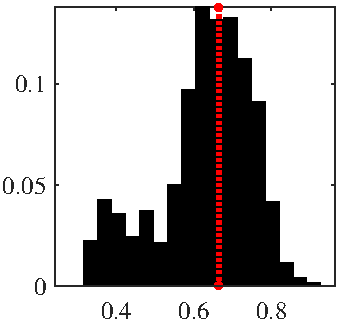
\includegraphics[scale=1]{dstats/CMD-adi-IAI.pdf}} \hspace{0.5cm} 
\subfloat[rupaka]{\label{fig:dstats:CMD:IAI:rupaka}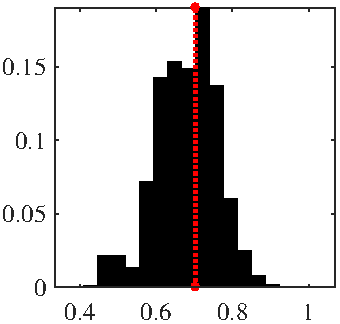
\includegraphics[scale=1]{dstats/CMD-rupaka-IAI.pdf}} \\ 
\subfloat[mishraChapu]{\label{fig:dstats:CMD:IAI:mishraChapu}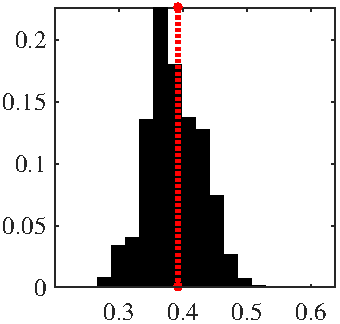
\includegraphics[scale=1]{dstats/CMD-mishraChapu-IAI.pdf}} \hspace{0.5cm} 
\subfloat[khandaChapu]{\label{fig:dstats:CMD:IAI:khandaChapu}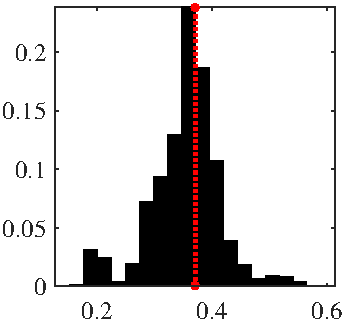
\includegraphics[scale=1]{dstats/CMD-khandaChapu-IAI.pdf}} \\ 
\caption[CMD-IAI]{CMD-IAI}\label{fig:dstats:CMD:IAI}
\end{center}
\end{figure}
%
%
% Dataset stats: CMDf-IAI
\begin{figure}[ht]
\captionsetup[subfigure]{labelformat=empty}
\begin{center}
\subfloat[adi]{\label{fig:dstats:CMDf:IAI:adi}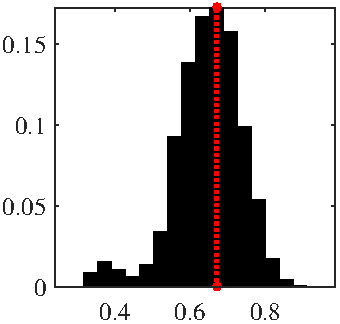
\includegraphics[scale=1]{dstats/CMDf-adi-IAI.pdf}} \hspace{0.5cm} 
\subfloat[rupaka]{\label{fig:dstats:CMDf:IAI:rupaka}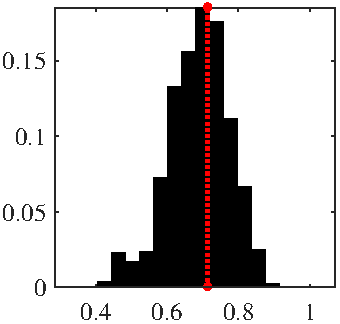
\includegraphics[scale=1]{dstats/CMDf-rupaka-IAI.pdf}} \\ 
\subfloat[mishraChapu]{\label{fig:dstats:CMDf:IAI:mishraChapu}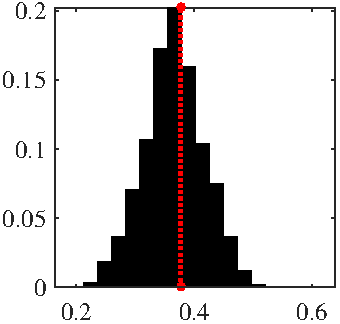
\includegraphics[scale=1]{dstats/CMDf-mishraChapu-IAI.pdf}} \hspace{0.5cm} 
\subfloat[khandaChapu]{\label{fig:dstats:CMDf:IAI:khandaChapu}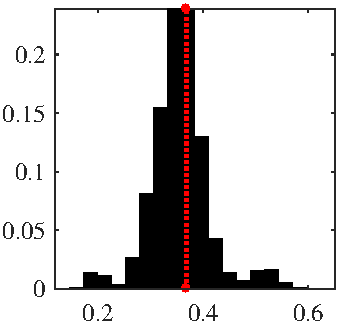
\includegraphics[scale=1]{dstats/CMDf-khandaChapu-IAI.pdf}} \\ 
\caption[CMDf-IAI]{CMDf-IAI}\label{fig:dstats:CMDf:IAI}
\end{center}
\end{figure}
%
%
% Dataset stats: HMDf-IAI
\begin{figure}[ht]
\captionsetup[subfigure]{labelformat=empty}
\begin{center}
\subfloat[teen]{\label{fig:dstats:HMDf:IAI:teen}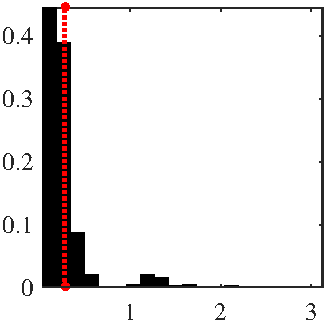
\includegraphics[scale=1]{dstats/HMDf-teen-IAI.pdf}} \hspace{0.5cm} 
\subfloat[ek]{\label{fig:dstats:HMDf:IAI:ek}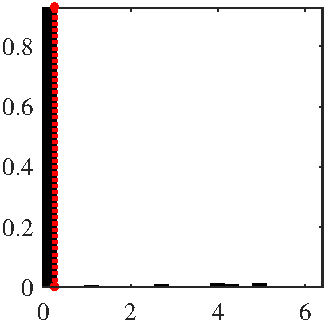
\includegraphics[scale=1]{dstats/HMDf-ek-IAI.pdf}} \\ 
\subfloat[jhap]{\label{fig:dstats:HMDf:IAI:jhap}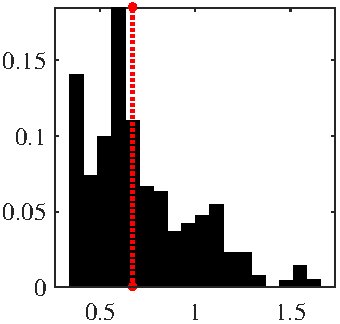
\includegraphics[scale=1]{dstats/HMDf-jhap-IAI.pdf}} \hspace{0.5cm} 
\subfloat[rupak]{\label{fig:dstats:HMDf:IAI:rupak}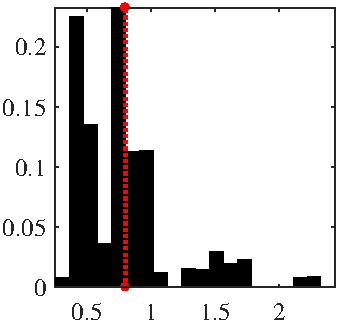
\includegraphics[scale=1]{dstats/HMDf-rupak-IAI.pdf}} \\ 
\caption[HMDf-IAI]{HMDf-IAI}\label{fig:dstats:HMDf:IAI}
\end{center}
\end{figure}
%
%
% Dataset stats: HMDl-IAI
\begin{figure}[ht]
\captionsetup[subfigure]{labelformat=empty}
\begin{center}
\subfloat[teen]{\label{fig:dstats:HMDl:IAI:teen}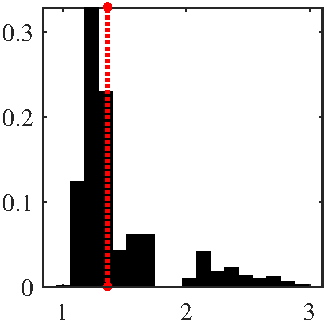
\includegraphics[scale=1]{dstats/HMDl-teen-IAI.pdf}} \hspace{0.5cm} 
\subfloat[ek]{\label{fig:dstats:HMDl:IAI:ek}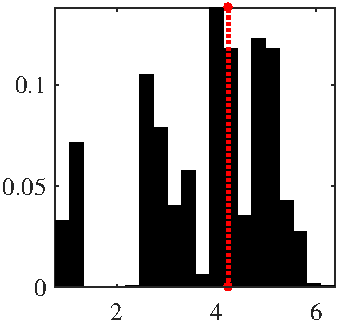
\includegraphics[scale=1]{dstats/HMDl-ek-IAI.pdf}} \\ 
\subfloat[jhap]{\label{fig:dstats:HMDl:IAI:jhap}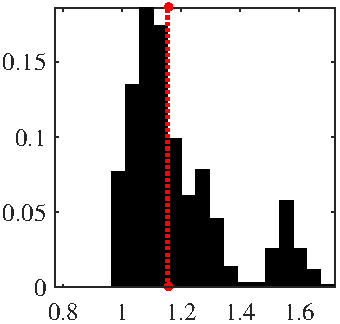
\includegraphics[scale=1]{dstats/HMDl-jhap-IAI.pdf}} \hspace{0.5cm} 
\subfloat[rupak]{\label{fig:dstats:HMDl:IAI:rupak}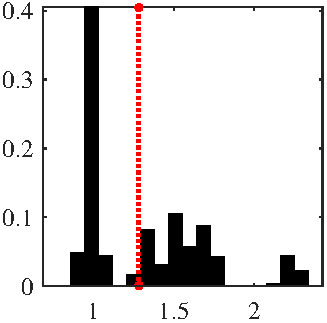
\includegraphics[scale=1]{dstats/HMDl-rupak-IAI.pdf}} \\ 
\caption[HMDl-IAI]{HMDl-IAI}\label{fig:dstats:HMDl:IAI}
\end{center}
\end{figure}
%
%
% Dataset stats: HMDs-IAI
\begin{figure}[ht]
\captionsetup[subfigure]{labelformat=empty}
\begin{center}
\subfloat[teen]{\label{fig:dstats:HMDs:IAI:teen}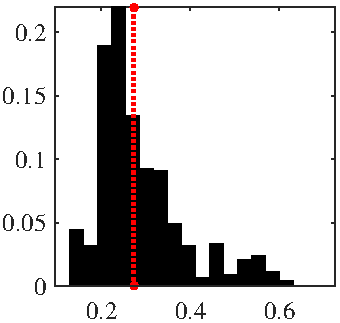
\includegraphics[scale=1]{dstats/HMDs-teen-IAI.pdf}} \hspace{0.5cm} 
\subfloat[ek]{\label{fig:dstats:HMDs:IAI:ek}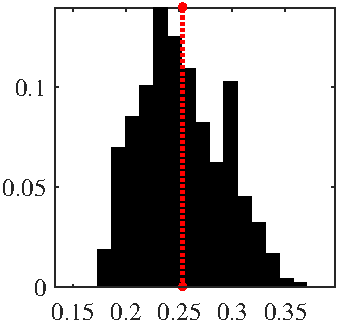
\includegraphics[scale=1]{dstats/HMDs-ek-IAI.pdf}} \\ 
\subfloat[jhap]{\label{fig:dstats:HMDs:IAI:jhap}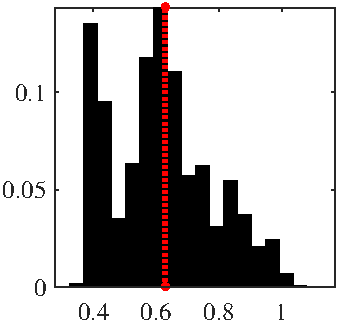
\includegraphics[scale=1]{dstats/HMDs-jhap-IAI.pdf}} \hspace{0.5cm} 
\subfloat[rupak]{\label{fig:dstats:HMDs:IAI:rupak}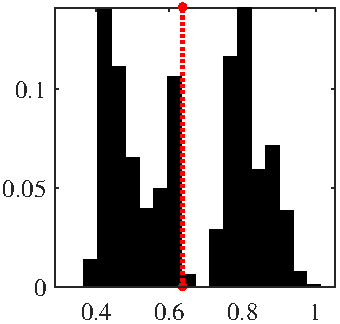
\includegraphics[scale=1]{dstats/HMDs-rupak-IAI.pdf}} \\ 
\caption[HMDs-IAI]{HMDs-IAI}\label{fig:dstats:HMDs:IAI}
\end{center}
\end{figure}
%
%
